\documentclass[12pt,a4paper]{article} \usepackage[spanish]{babel} \usepackage{graphicx} \usepackage{amsmath} \usepackage{amsfonts} \usepackage{amssymb} \usepackage{float} \usepackage{geometry}

% Configuración de márgenes \geometry{ left=2cm, right=2cm, top=2.5cm, bottom=2.5cm }

\title{\textbf{Análisis de estrategias de negocios en la industria hotelera a través de la simulación computacional de un hotel}}
\author{Massiel Paz Otaño -\ estudiante de 3er año de Ciencia de la Computación, \\ Facultad de Matemática y Computación, Universidad de La Habana\\\\ Marlon Díaz Pérez -\ estudiante de 3er año de Ciencia de la Computación, \\ Facultad de Matemática y Computación, Universidad de La Habana\\\\ Albaro Suárez Valdés -\ estudiante de 3er año de Ciencia de la Computación, \\ Facultad de Matemática y Computación, Universidad de La Habana} \date{1ro de septiembre de 2024}
\begin{document}

\maketitle

\vspace{-1em} \hrulefill

\section*{Resumen y Abstract}

\subsection*{Resumen} \addcontentsline{toc}{section}{Resumen}

Este trabajo presenta una simulación computacional de un hotel, basada en agentes inteligentes, con el objetivo de evaluar la eficacia de diferentes estrategias de negocio en el ámbito hotelero. La simulación contempla tres tipos de agentes fundamentales: turistas, trabajadores y el gerente del hotel. Los turistas tienen, entre otros aspectos, una serie de restricciones que deben cumplir las habitaciones en las que se alojarán. Para lograr su cumplimiento, se aplica el algoritmo de Constraint Satisfaction Problem (CSP). El gerente es quien implementa las distintas estrategias, conocidas en el sector hotelero, a partir de las reacciones de los turistas, utilizando algoritmos de inteligencia artificial. Se emplea una metaheurística para determinar qué servicios conviene añadir al hotel con el fin de optimizar las ganancias. Se compararon dos criterios de parada para este algoritmo, donde se concluyó que el criterio de parada por cantudad de iteraciones daba mejores resultados.

Paralelamente, se realiza un estudio que involucra la generación y clasificación de reseñas por un Large Language Model (LLM), a partir de las reacciones de los turistas motivadas por sus experiencias. Las clasificaciones se compararon con el nivel de satisfacción real de cada turista, obteniéndose resultados diferentes, en su mayoría, y con poca varianza. Además, se analizó la relación entre la satisfacción de cada turista y la calidad de los servicios.

\subsection*{Palabras clave} \textit{Simulación, Agentes Inteligentes, Estrategias de Negocio, Algoritmos de IA, LLM}

\subsection*{Abstract} This work presents a computational simulation of a hotel, based on intelligent agents, with the aim of evaluating the effectiveness of different business strategies in the hotel field. The simulation contemplates three types of fundamental agents: tourists, workers and the hotel manager. Tourists have, among other aspects, a series of restrictions that must be met by the rooms in which they will stay. To achieve compliance, the Constraint Satisfaction Problem (CSP) algorithm is applied. The manager is the one who implements the different strategies, known in the hotel sector, based on the reactions of tourists, using artificial intelligence algorithms. A metaheuristic is used to determine which services should be added to the hotel in order to optimize profits. Two stop criteria for this algorithm were compared, where it was concluded that the stop criterion by number of iterations gave better results. 

At the same time, a study is carried out that involves the generation and classification of reviews by a Large Language Model (LLM), based on the reactions of tourists motivated by their experiences. The rankings were compared with the level of real satisfaction of each tourist, obtaining different results, for the most part, and with little variance. In addition, the relationship between the satisfaction of each tourist and the quality of services was analyzed.

\subsection*{Keywords}\textit{1. Hotel Simulation, Intelligent Agents, Business Strategies, Large Language Model (LLM)}

\vspace{-1em} \hrulefill

\section{Introducción}

La industria hotelera se encuentra en constante evolución, buscando optimizar sus operaciones y estrategias para satisfacer las necesidades cambiantes de los viajeros. En este contexto, la simulación computacional ha surgido como una herramienta poderosa para analizar y evaluar diferentes escenarios de negocio. Este trabajo presenta una simulación de un hotel basada en agentes inteligentes, la cual constituye la base sobre la que se desarrollan los estudios de este trabajo.

Este trabajo se centra en la interacción entre tres tipos de agentes: turistas, personal del hotel y el gerente; y el medio: el hotel. Los clientes, con sus preferencias y limitaciones individuales, interactúan con el hotel, buscando satisfacer sus necesidades. Los trabajadores se encargan de cumplir con sus deberes en sus respectivas labores, haciendo depender su eficacia del salario que reciben. El gerente, por su parte, toma decisiones estratégicas para optimizar la rentabilidad del hotel, basándose en el comportamiento de los clientes y utilizando algoritmos de inteligencia artificial para identificar las mejores opciones.

El hotel, como medio en el que se desarrolla la simulación, contiene los recursos necesarios para que los agentes puedan modificarlo, así como consultar el estado de sus propiedades, en dependencia del rol que estén desenvolviendo. Los agentes, a su vez, se verán influenciados por el medio, donde dicha afectación dependerá principalmente de las creencias de cada uno.

El objetivo principal de este trabajo es evaluar la eficacia de diferentes estrategias de negocio en el ámbito hotelero, así como la realización de otros estudios sobre los datos obtenidos y eficiencia de algunos de los algoritmos utilizados de inteligencia artificial (IA). Se busca analizar la influencia de las estrategias de gestión en la satisfacción del cliente, la eficiencia del hotel y la rentabilidad del negocio. Además, se realiza un estudio paralelo utilizando un Modelo de Lenguaje de Gran Escala (LLM) para analizar la relación entre las experiencias de los clientes y las reseñas que generan, y de esta forma determinar si la percepción de los clientes, reflejada en las reseñas, se corresponde con su satisfacción real.

\section{Marco teórico}

Presenta aquí una revisión crítica de la literatura existente sobre el tema, conceptos clave relacionados con el objeto de estudio, y teorías relevantes que sustentan la investigación.

\section{Método}

Para los estudios realizados en este trabajo, se tiene como principal herramienta y método de generación y obtención de datos, la simulación computacional conformada para este trabajo en particular en el lenguaje de programación Python. Por esta razón, es necesario conocer los detalles de su implementación.

\subsection{Simulación}
Esta, es una simulación basada en agentes inteligentes que interactúan entre sí y con el medio, cuyas implementaciones serán abordadas en las secciones posteriores. Como el objetivo es analizar la influencia de varias estrategias de negocio en la satisfacción de los turistas, lo cual influye directamente en las ganancias del hotel, se hace evidente la presencia del factor tiempo, por tanto, la simulación conformada es dinámica.\\
Para controlar el flujo de la simulación, así como la creación y uso de procesos, y activación de eventos, se usó la biblioteca \textbf{simpy} de python.

\subsubsection{Medio}
Dado que se dessarrolla en un hotel, el medio en el que se desarrolla la simulación es, justamente, un hotel. Representado computacionalmente por una clase, el hotel posee distintas propiedades y métodos que brindan información y permiten su utilización a los agentes que con él interectúen.\\
Cabe destacar, además, las clases \textit{Service} y \textit{Utility} que permiten obtener detalles de los servicios que ofrece el hotel, por ejemplo: precio, costo y estado de mantenimiento, utilidades que incluye, necesidad particular que satisface (por ejemplo, el restaurante satisface el hambre), entre otros. Las utilidades, por su parte, pertenecen siempre a un servicio, y también contienen su propia información.

\subsubsection{Agentes}
En esta simulación intervienen 3 "tipos" diferentes de agentes: los turistas, los trabajadores y el gerente del hotel. Todos los agentes poseen una arquitectura Beliefs Desires Intentions (BDI) que les permite tomar decisiones a partir de sus propios intereses y las circunstancias externas.\\ 
Los turistas buscan satisfacer sus necesidades (sueño, hambre, diversión y confort) a través del uso de los servicios y utilidades del hotel, en cuya calidad interviene directamente los trabajadores de cada servicio ofrecido. Asimismo, los turistas poseen una serie de restricciones, características o comodidades que debe tener las habitaciones en las que se hospedarán.\\
Los trabajadores, por su parte, realizan sus labores con un nivel de eficacia y rapidez equivalente a su salario.\\
Por último, el gerente del hotel se encarga de aplicar estrategias de negocio con el fin de satisfacer de una mejor forma las necesidades de la mayoría de los turistas teniendo en cuenta las características y restricciones del medio: presupuesto, ganancias, temporada alta o baja, entre otros, con el fin de maximizar las ganancias.

\subsection{Inteligencia Artificial (IA)}
El uso de algoritmos de inteligencia artificial en este trabajo resultó crucial para el cumplimiento de los objetivos e estudio. A continuación se expondrán los algoritmos utilizados y con qué fin.

\subsubsection{Constraint Satisfaction Problem (CSP)}
Anteriormente se mencionó que los turistas imponían una serie de restricciones que deben tener las habitaciones en las cuales se hospeden. Las habitaciones, como es lógico, también poseen determinadas características que pueden o no coincidir con aquellas que el turista desee. Para resolver el problema de buscar cuál es la mejor forma de asignar habitaciones a un conjunto de turistas, a modo de complacer a la mayor cantidad de turistas, se empleó el algoritmo Constraint Satisfaction Problem (CSP). Obsérvese que el espacio sobre el cual se realiza la búsqueda crece exponencialmente, por tanto resulta inviable resolver dicho problema con algún otro algoritmo que no incluya inteligencia artificial.

\subsubsection{Metaheurística}
Uno de las estrategias de negocio que aplica el gerente en aras de hacer crecer las ganancias, es la inclusión de nuevos servicios en el hotel. Sin embargo, es necesario tener en cuenta el presupuesto disponible, así como el costo de añadir dicho servicio (costo de construcción, y de contratación de empleados) así como las ganancias que se esperan obtener una vez se active. Con el objetivo de contrar la mejor combinación de servicios a añadir que maximicen las ganancias se empleó un algoritmo de metaheurística, al ser un problema de optimización en un espacio de búsqueda (verificar acá lo del espacio de búsqueda)

\subsubsection{Large Language Model (LLM)}
Cuando cada turista utiliza un servicio o utilidad, añade a su cúmulo de experiencias un frase breve que clasifica el servicio. Luego todo este conjunto de frases son procesadas por un LLM para generar una reseña coherentemente redactada. Luego, esta reseña será analizada por el propio LLM el cual la utilizará para clasificar en: 'Excellent' (excelente), 'Very Good' (muy buena), 'Good' (buena), 'Bad' (mala) o 'Very Bad' (muy mala) la experiencia de un turista. Cabe destacar que el cálculo real de la satisfacción del turista existe, y se realiza a partir de sus experiencias propias.

\subsection{Estudios}
\subsubsection{Cambiando el criterio de parada}
Una de las estrategias de negocio aplicadas por el gerente consiste en añadir nuevos servicios al hotel. Su elección buscará maximizar la ganancia, por lo que agregará el conjunto de servicios que satisfaga esta condición. Para ello se empleó una metaheurística (explicado anteriormente) cuyo criterio de parada consiste en un límite, es decir, una vez que se alcance una ganancia objetivo, se aprueba como conjunto de servicios válido a añadir. Sin embargo, ¿las ganancias obtenidas se mantendrá si utilizamos como criterio de parada la cantidad de iteraciones del algoritmo? Para responder a esta interrogante se realizó 100 simulaciones con cada criterio, y luego se hizo una prueba de Mann-Whitney U para analizar la varianza entre las ganancias. Los resultados y discusión serán expuestos en la próxima sección.\\
\subsubsection{Servicio más popular y servicio que reporta mayores ganancias}
Resulta necesario para el negocio de la hotelería saber cuál es el servicio más usado por los huéspedes así como el que reporta mayores ganancias. Con 100 simulaciones realizadas aplicando un criterio de parada, y luego 100 simulaciones más aplicando el otro criterio de parada, se analizó asimismo si el servicio más popular y el que reporta mayor ganancia están relacionados con este cambio en el algoritmo de metaheurística.
\subsubsection{Análisis de la influencia en las ganancias que tienen las estrategias tomadas por el gerente}
Es necesario saber si las estrategias tomadas por el manager implican algún cambio positiva en las ganancias del hotel. Para este análisis, primero se realizaron 100 simulaciones donde la única regla del gerente es mantener el nivel de mantenimiento (valga la redundancia) de los servicios en un porciento aceptable. En otras 100 simulaciones el manager ha tomado todas las estrategis que ha considerado en base a sus reglas de negocio. De cada experimento se almacenan las ganancias obtenidas y se realiza una prueba de Mann-Whitney U para analizar las diferencias entre ellas.\\

\subsubsection{Clasificación del LLM vs experiencia real}
En este trabajo se ha usado un LLM en dos fases: 1ro, dado un conjunto de frases que el turista devuelve de acuerdo a su experiencia en el hotel, el LLM genera una reseña coherente que corresponde a ese turista; 2do, el mismo LLM (pero ahora en calidad de clasificador) asignará, en base a la reseña generada, una etiqueta que clasificará la experiencia del turista en: 'Excellent' (excelente), 'Very good' (muy buena), 'Good' (buena), 'Mala' (bad) o 'Very bad' (muy mala). Cada una de estas clasificaciones corresponden a un rango numérico comprendido entre 0 y 100 ( $80 < x \le 100$: Excellent, $60 < x \le 80$: Very Good, $40 < x \le 60$: Good, $20 < x \le 40$: Bad, $0 \le x \le 20$: Very bad), para que pueda compararse con la experiencia real del turista, cuyo cálculo arroja un número, justamente, entre 0 y 100.\\
Por una cuestión de tiempo de ejecución, se decidió realizar solo 10 simulaciones para este estudio, dado que el algoritmo de un LLM demora en ejecutarse. Para medir la varianza entre las clasificaciones del LLM y la satisfacción real de los turistas, se usó un test de ANOVA (realizar otro test para la varianza o realizar el análisis de los supuestos para ANOVA). Se realizó, además, un test de correlación de Spearman para analizar la relación existente entre la clasificación del LLM y la satisfacción real.
\subsubsection{Relación experiencia del turista con calidad de servicio del hotel}
Además se realizó un estudio para verificar si existía una correlación entre la calidad de los servicios del hotel y el nivel de satisfacción de los turistas. Para ello se utilizó el test de correlación de Spearman y se analizó la correctitud del cálculo de la satisfacción de los turistas.


\section{Resultados y discusión}

%Presenta sistemáticamente los hallazgos obtenidos. Puedes incluir aquí tablas, gráficos y figuras que ilustren los resultados principales.
%Interpreta los resultados en relación con las hipótesis planteadas, compara con estudios previos similares y discute las implicaciones prácticas y teóricas de los hallazgos.

\subsubsection{Cambiando el criterio de parada}

\begin{figure}[H] \centering \includegraphics[width=\textwidth]{Distribución de ganancias por estrategia} \caption{} \label{fig:etiqueta} \end{figure}

Para este análisis se tomaron como hipótesis nula y alternativas las siguientes:\\
$H_0$: No hay diferencia entre las medias de las ganancias producidas aplicando cada criterio.\\
$H_1$: Hay diferencia entre las medias de las ganancias producidas aplicando cada criterio.\\
\textbf{Prueba de Mann-Whitney U:}\\
\textit{Estadístico U:} 2646.0\\
\textit{Valor p:} 8.897161660760197e-09\\
En la gráfica se puede apreciar que la estrategia que aplica el criterio de parada por cantidad de iteraciones reporta mayores ganancias que la que aplica el criterio por umbral. Ahora, al obtenerse un valor del estadístico U alto, tomando $\alpha$ = 0.05, resulta que $\alpha$ < p-value = 8.897161660760197e-09, luego, efectivamente, existe una diferencia significativa en la ganancia entre las estrategias, por tanto se rechaza la hipótesis nula de que no hay diferencia. Podemos asegurar que la estrategia que produjo los datos con mayor media es mejor, en este caso es la que posee el criterio de parada por \textbf{cantidad de iteraciones} con una ganancia media de 15689.76 aproximadamente.
\subsubsection{Servicio más popular y servicio que reporta mayores ganancias}
\begin{figure}[H] \centering 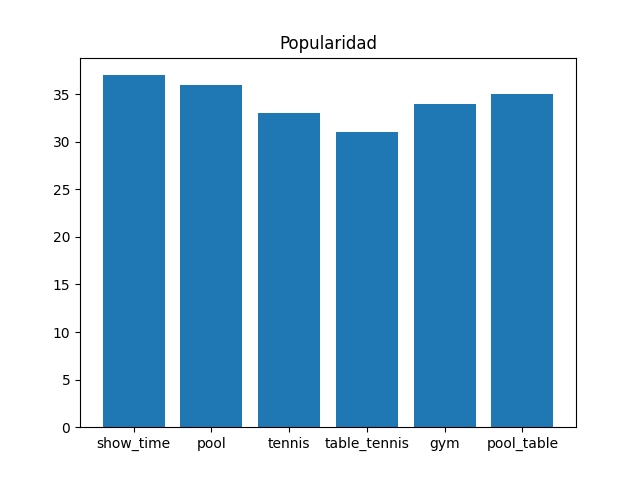
\includegraphics[width=\textwidth]{Popularidad serv} \caption{Servicios más populares} \label{fig:etiqueta} \end{figure}
\begin{figure}[H] \centering 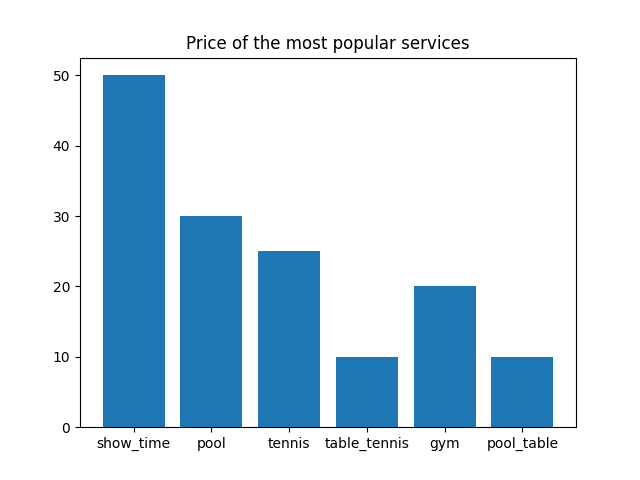
\includegraphics[width=\textwidth]{precio popularidad} \caption{Precios de los servicios más populares} \label{fig:etiqueta} \end{figure}
\begin{figure}[H] \centering \includegraphics[width=\textwidth]{Mayor Ganancia} \caption{Servicios con mayor ganancia} \label{fig:etiqueta} \end{figure}
\begin{figure}[H] \centering \includegraphics[width=\textwidth]{precio mayor ganancia} \caption{precios de los servicios con mayor ganancia} \label{fig:etiqueta} \end{figure}
Como se ilustran en las gráficas, se puede decir que los 5 servicios más utilizados por los turistas son (ver Figura 2)  y los que reportan mayores ganancias son (ver Figura 4) Resulta evidente percatarse que los servicios que pertenecen a dichas categorías no tienen por qué coincidir. Si se analiza, además, las gráficas que ilustran los precios de los servicios más populares así como los que reportan mayores ganancias, es posible distinguir que que el precio de estos últimos es más que el doble de los primeros. Esto podría sugerir que el precio de los servicios influye en las ganancias que reporten al hotel, considerablemente más que su nivel de popularidad entre los clientes.
\subsubsection{Análisis de la influencia en las ganancias que tienen las estrategias tomadas por el gerente}
\begin{figure}[H] \centering 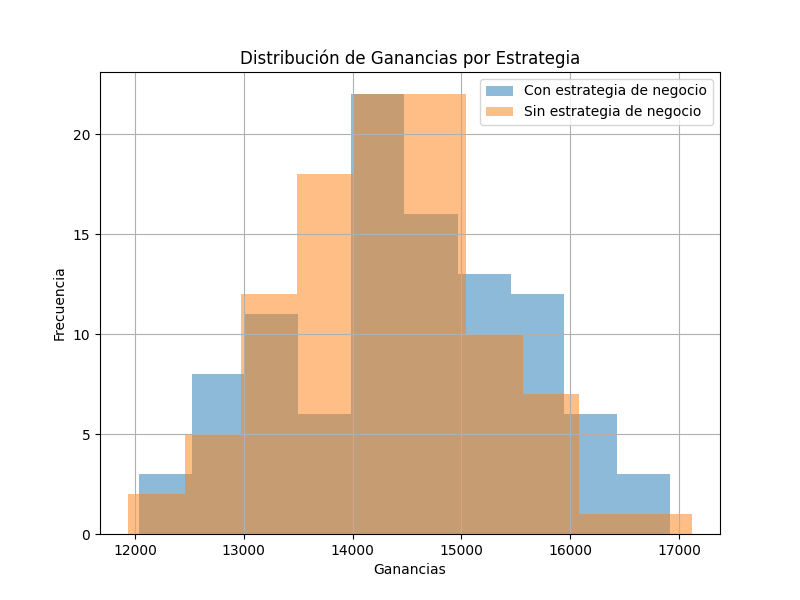
\includegraphics[width=\textwidth]{estrategias manager} \caption{Ganancia con y sin estrategias de negocio} \label{fig:etiqueta} \end{figure}

Para este análisis se tomaron como hipótesis nula y alternativas las siguientes:\\
$H_0$: No hay diferencia entre las medias de las ganancias producidas con y sin aplicar las estrategias del gerente.\\
$H_1$: Hay diferencia entre las medias de las ganancias producidas con y sin aplicar las estrategias del gerente.\\
\textbf{Prueba de Mann-Whitney U:}\\
\textit{Estadístico U:} 5598.0\\
\textit{Valor p:} 0.14431042503881425\\
Ganancia media generada por las estrategias del manager: 14485.1443\\
Ganancia media obtenida sin las estrategias del manager: 14290.28.\\

Como se puede apreciar en la gráfica, es casi imperceptible la diferencia entre las ganancias reportadas al aplicar solo la estrategia de sostener un nivel de mantenimiento aceptable en los servicios, respecto a las generadas por la suma de aplicar las otras estrategias.\\

Respecto a los resultados de la prueba de Mann-Whitney U, se puede apreciar un estadístico U con un valor elevado, sin embargo, tomando $\alpha$ = 0.05, se tiene que p-value > $\alpha$, luego no hay evidencia suficiente para rechazar la hipótesis nula, por tanto no se puede afirmar estadísticamente que hay una evidencia significatiova entre las ganancias obtenidas al aplicar o no, las estrategias del gerente. Por lo tanto, no es posible concluir que las estrategias tomadas por el manager son mejores en cuanto a ganancias reportadas que aquella que solo contempla el mantenimiento de los servicios.\\
Dado que este resultado es un poco extraño, resulta conveniente revisar o bien las estrategias y reglas del gerente, o bien el cálculo de las ganancias en la simulación.

\subsubsection{Clasificación del LLM vs experiencia real}
\begin{figure}[H] \centering 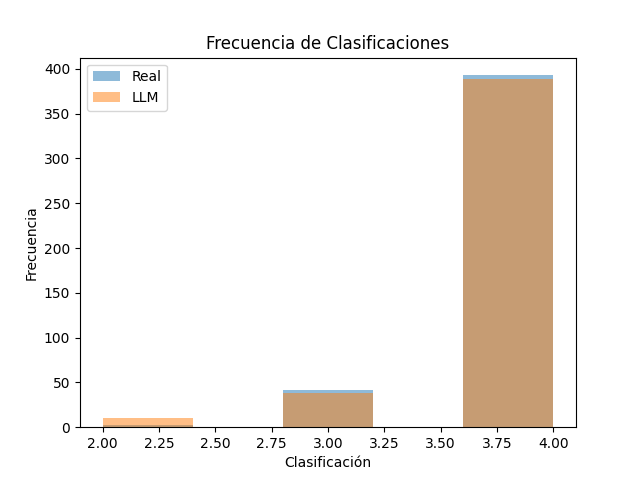
\includegraphics[width=\textwidth]{Frecuencia de clasificaciones_last} \caption{frecuencia de clasif} \label{fig:etiqueta} \end{figure}
En esta gráfica se puede apreciar que se realizaron más de 400 clasificaciones (más de 400 turistas), donde las barras correspondientes a cada clasificación, la del LLM y la correspondiente al cálculo real prácticamente se solapan.
\begin{figure}[H] \centering 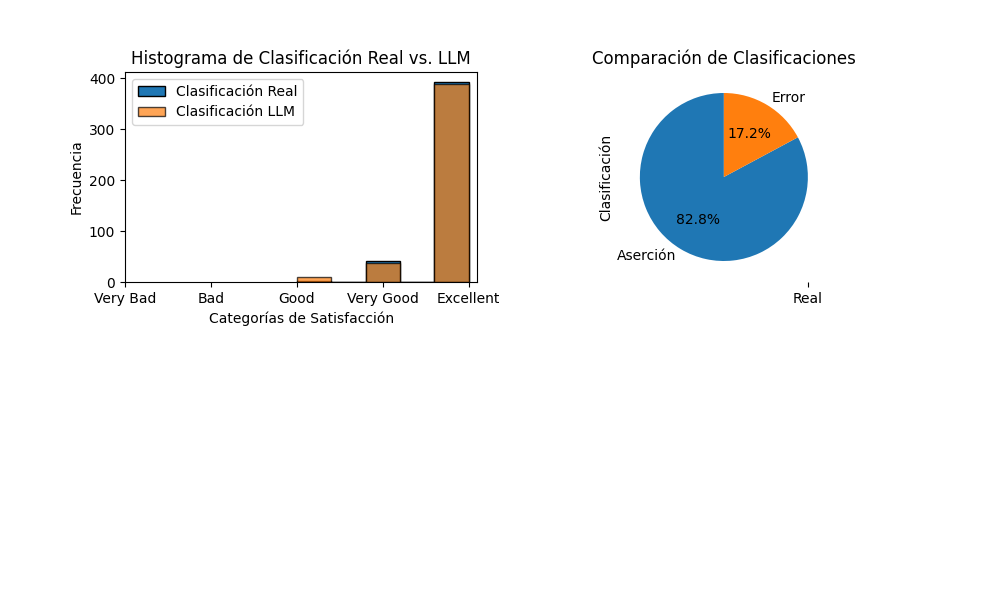
\includegraphics[width=\textwidth]{LLM classif vs real satisfaction_last} \caption{errores LLM} \label{fig:etiqueta} \end{figure}
En esta gráfica se puede apreciar que el LLM prácticamente coincidió en su clasificación con el resultado del cálculo de la satisfacción de los turistas, acertando un 82,2\% del total de clasificaciones. Ahora, analicemos cuánta diferencia hay entre ambas clasificaciones.
\begin{figure}[H] \centering 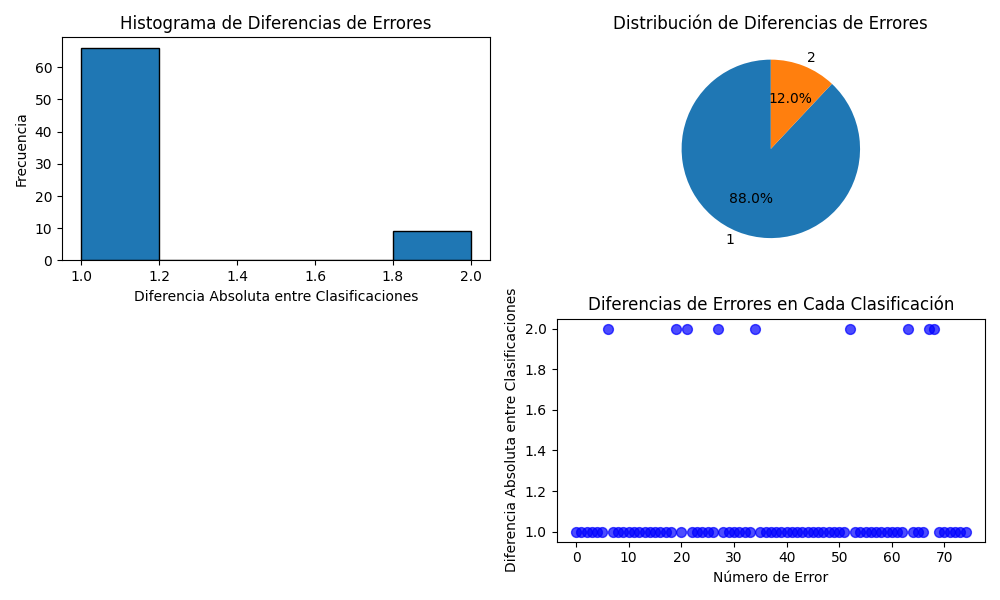
\includegraphics[width=\textwidth]{Diferencia de errores_last} \caption{diferencia entre errores} \label{fig:etiqueta}\end{figure}
A partir de esta gráfica se puede apreciar que la mayoría de las clasificaciones dadas por el LLM, dista 1 unidad de la claseificación real. Dado que son 5 clasificaciones en total, se puede inferir que el margen de error no es estadísticamente significativo.

\textbf{Correlación de Spearman entre Clasificación Real y del LLM:}\\
0.127 (P-value: 0.008)\\
Dado que la correlación es de 0.127 (débil por ser cercana a 0), y p-value = 0.008 $< \alpha$ = 0.05, se puede afirmar que existe evidencia suficiente para rechazar la hipótesis nula de que no existe conrrelación entre las variables. Este resultado indica que las clasificaciones, efectivamente, están coincidiendo.

\subsubsection{Relación experiencia del turista con calidad de servicio del hotel} %Mejorar esta vaina
\begin{figure}[H] \centering \includegraphics[width=\textwidth]{Clasificación real y nivel de servicios_last} \caption{clasificación real vs nivel de los servicios} \label{fig:etiqueta} \end{figure}
Correlación de Spearman entre Clasificación Real y Nivel de Servicios: -0.047 (P-value: 0.325)\\
Debido al bajo nivel de correlación y al valor del p-value = 0.325 $> \alpha$ = 0.05, se puede concluir que no existe evidencia suficiente para rechazar la hipótesis nula de que no existe correlación entre la calidad de los servicios y el nivel de satisfacción de los turistas. Esta conclusión resulta un poco rara, pues la segunda debería estar altamente influenciadaa por la primera.


\section{Conclusiones}

%Resume concisamente los principales hallazgos, indica si se cumplieron los objetivos propuestos y menciona las limitaciones del estudio.
La simulación computacional basada en agentes inteligentes ha demostrado ser una herramienta útil para evaluar la eficacia de diferentes estrategias de gestión hotelera. Los resultados sugieren que las estrategias de gestión impactan significativamente en la satisfacción del cliente (valorar la posibilidad de añadir este estudio), la eficiencia del hotel y la rentabilidad del negocio. El estudio con el Large Language Model (LLM) indica que la percepción de los clientes, reflejada en las reseñas, no siempre se corresponde con su satisfacción real. Se recomienda profundizar en la investigación utilizando un mayor número de variables y estrategias, así como explorar la aplicación de técnicas de aprendizaje automático y análisis predictivo en la gestión hotelera.

\section{Recomendaciones}

Para acercar los resultados obtenidos en esta simulación a los que se pueden obtener en la vida real se recomienda ajustar la escala de tiempo. Asimismo sería interesante analizar la influencia de las diferentes estrategias de marketing vía digital en el desarrollo del hotel, principalmente en la llegada de los clientes.


\end{document} $